\documentclass[11pt,a4paper]{article}

% === Font & encoding (XeLaTeX) ===
\usepackage{fontspec}
\setmainfont{Latin Modern Roman}
\setsansfont{Latin Modern Sans}
\setmonofont{Latin Modern Mono}

% Korean font support via ucharclasses
\usepackage{ucharclasses}
\newfontfamily\koreanfont{Droid Sans Fallback}[Scale=0.95]
\setTransitionsForCJK{\koreanfont}{\setmainfont{Latin Modern Roman}}

% === Layout ===
\usepackage[margin=2cm,headheight=14pt]{geometry}
\usepackage{graphicx}
\usepackage{booktabs}
\usepackage{longtable}
\usepackage{float}
\usepackage{hyperref}
\usepackage{xcolor}
\usepackage{fancyhdr}
\usepackage{titlesec}
\usepackage{caption}
\usepackage{multirow}
\usepackage{enumitem}
\usepackage{array}
\usepackage{tabularx}
\usepackage{amssymb}

% === Header/Footer ===
\pagestyle{fancy}
\fancyhf{}
\rhead{V9 Cross-Model SAE Analysis}
\lhead{LLM Gambling Addiction}
\cfoot{\thepage}

% === Section styling ===
\titleformat{\section}{\Large\bfseries}{\thesection}{1em}{}
\titleformat{\subsection}{\large\bfseries}{\thesubsection}{1em}{}
\titleformat{\subsubsection}{\normalsize\bfseries}{\thesubsubsection}{1em}{}

% === Hyperlinks ===
\hypersetup{
    colorlinks=true,
    linkcolor=blue!60!black,
    citecolor=green!50!black,
    urlcolor=blue!70!black
}

% === Title ===
\title{\textbf{V9: Cross-Model, Cross-Domain Neural Basis of\\Risky Decision-Making in LLMs}\\[0.5em]
\large Internal Research Report (v9.5)\\[0.3em]
\normalsize ``Can Large Language Models Develop Gambling Addiction?''}
\author{Seungpil Lee, Donghyeon Shin, Yunjeong Lee, Sundong Kim\\
\small GIST (Gwangju Institute of Science and Technology)}
\date{March 19, 2026}

\begin{document}
\maketitle
\tableofcontents
\newpage

% ============================================================
% METADATA
% ============================================================
\noindent\textbf{Models}: Gemma-2-9B-IT (42L, 3584-dim, GemmaScope 131K) $|$ LLaMA-3.1-8B-Instruct (32L, 4096-dim, LlamaScope 32K)\\
\textbf{Paradigms}: Investment Choice (IC, 1600 games), Slot Machine (SM, 3200 games), Mystery Wheel (MW, 3200 games)\\
\textbf{Data}: Gemma: IC+SM+MW; LLaMA: IC+SM (MW pending)\\
\textbf{Pipeline}: StandardScaler $\rightarrow$ PCA(50) $\rightarrow$ LogReg(C=1.0, balanced) $|$ 5-fold StratifiedKFold

\medskip\noindent\textit{Data integrity: All numerical claims are traceable to computed JSON outputs.}

\bigskip\hrule\bigskip

% ============================================================
% CENTRAL QUESTION
% ============================================================
\section*{Central Question}
\addcontentsline{toc}{section}{Central Question}

\textbf{Do different models, across different gambling tasks, under different prompt conditions, share a common neural basis for bankruptcy --- the most extreme risk outcome?}

\begin{itemize}[nosep]
    \item \textbf{RQ1}: Do Gemma and LLaMA share common activation/feature patterns that predict bankruptcy?
    \item \textbf{RQ2}: Do activation patterns remain invariant when the domain (IC, SM, MW) changes?
    \item \textbf{RQ3}: Are neural representations consistent across prompt conditions (Fixed/Variable, G/M/W/P/R)?
\end{itemize}

% ============================================================
% EXECUTIVE SUMMARY
% ============================================================
\section*{Executive Summary}
\addcontentsline{toc}{section}{Executive Summary}

\textbf{RQ1 --- Universal BK Features Exist Across Architectures.}
600 of 3,584 Gemma L22 neurons (16.7\%) are sign-consistent universal BK predictors across three paradigms (FDR $p<0.01$). 744 SAE features across 7 layers show cross-domain consistency (L18+ binomial $p<5\times10^{-3}$). LLaMA achieves near-identical BK classification (AUC 0.974 vs Gemma 0.976 in SM). Factor decomposition confirms 65--71\% of SAE features encode BK independently of bet-type and paradigm (permutation $p=0.000$, null $\sim$1\%).

\medskip\textbf{RQ2 --- Strong Domain Invariance (Gemma), Selective Invariance (LLaMA).}
Gemma cross-domain transfer reaches AUC 0.87--0.93 (IC$\rightarrow$MW, SM$\rightarrow$MW; all $p=0.000$). A 3D shared BK subspace achieves AUC 0.86--0.97 despite near-orthogonal LR weight vectors. LLaMA IC$\rightarrow$SM transfer succeeds only at L25 (AUC 0.783), while SM$\rightarrow$IC is more stable (AUC 0.685 at L30). Hidden state transfer exceeds SAE transfer by 0.10--0.25 in most directions.

\medskip\textbf{RQ3 --- BK Representation Is Condition-Invariant, but Condition Effects Are Model-Dependent.}
LLaMA IC shows $\cos>0.81$ between Variable and Fixed BK directions across all layers ($n\ge65$ per group). Both models have $\sim$33--37\% shared BK neurons. G(Goal) dominates BK behaviorally in Gemma ($20.75\times$) but not LLaMA ($1.26\times$), yet both share the mechanism: G drives BK independently without modulating existing BK representations.

\bigskip\hrule\bigskip

% ============================================================
% 1. SETUP
% ============================================================
\section{Setup}

\subsection{Data \& Representations}

\begin{table}[H]
\centering
\caption{Dataset Overview}\label{tab:dataset}
\footnotesize
\begin{tabular}{lccclll}
\toprule
Paradigm & Games & BK & BK\% & Bet Types & Constraints & Prompt Cond. \\
\midrule
IC (Gemma)  & 1,600 & 172   & 10.8\% & Fixed/Var & c10/c30/c50/c70 & BASE/G/M/GM \\
SM (Gemma)  & 3,200 & 87    & 2.7\%  & Fixed/Var & \$10 fixed      & 32 combos \\
MW (Gemma)  & 3,200 & 54    & 1.7\%  & Fixed/Var & \$30 fixed      & 32 combos \\
IC (LLaMA)  & 1,600 & 142   & 8.9\%  & Fixed/Var & c10/c30/c50/c70 & BASE/G/M/GM \\
SM (LLaMA)  & 3,200 & 1,164 & 36.4\% & Fixed/Var & \$10 fixed      & 32 combos \\
\bottomrule
\end{tabular}
\end{table}

\subsection{V8 Limitations Addressed}

V8 (Gemma-only) left three weaknesses:
\begin{enumerate}[nosep]
    \item \textbf{SAE cross-domain failure}: Only 1/131K features was sign-consistent at L22 top-50. V9: \textbf{744 features} across 7 layers (\S\ref{sec:sae744}).
    \item \textbf{Variable/Fixed ``dissociation''}: Artifact of comparing all games, not BK-only (\S\ref{sec:bkdir}).
    \item \textbf{Single model}: V9 adds LLaMA IC+SM (\S\ref{sec:crossmodel}, \S\ref{sec:llamatransfer}).
\end{enumerate}

\subsection{Cross-Model BK Rate Asymmetry}

\begin{table}[H]
\centering
\caption{BK Rate Asymmetry Between Models}\label{tab:bk_asymmetry}
\footnotesize
\begin{tabular}{lcccc}
\toprule
 & Gemma IC & LLaMA IC & Gemma SM & LLaMA SM \\
\midrule
Fixed BK rate    & \textbf{19.75\%} & 8.1\%  & --- & --- \\
Variable BK rate & 1.75\%  & \textbf{9.6\%}  & --- & --- \\
Overall BK rate  & 10.8\%  & 8.9\%  & 2.7\%  & \textbf{36.4\%} \\
Autonomy effect  & $-$18.0pp & $+$1.5pp & --- & --- \\
\bottomrule
\end{tabular}
\end{table}

% ============================================================
% 2. RQ1
% ============================================================
\section{RQ1: Universal BK Features}

\subsection{600 Universal BK Neurons (Gemma L22)}

Point-biserial correlation per neuron per paradigm, FDR-corrected (BH, $p<0.01$). Neurons significant in all three paradigms with consistent sign are ``Universal BK Neurons.''

\begin{table}[H]
\centering
\caption{Universal BK Neuron Summary (Gemma L22)}\label{tab:universal}
\footnotesize
\begin{tabular}{lcccc}
\toprule
 & IC & SM & MW & Cross-paradigm \\
\midrule
FDR-significant     & 2,528 (70.5\%) & 2,725 (76.0\%) & 2,314 (64.6\%) & --- \\
All-3-significant   & --- & --- & --- & 1,238 (34.5\%) \\
\textbf{Sign-consistent} & --- & --- & --- & \textbf{600 (16.7\%)} \\
BK-promoting        & --- & --- & --- & 302 \\
BK-inhibiting       & --- & --- & --- & 298 \\
\bottomrule
\end{tabular}
\end{table}

\begin{table}[H]
\centering
\caption{Top-5 Universal BK Neurons}\label{tab:top5}
\footnotesize
\begin{tabular}{ccccccl}
\toprule
Rank & Neuron & min$|r|$ & IC $r$ & SM $r$ & MW $r$ & Direction \\
\midrule
1 & \textbf{1763} & 0.217 & +0.305 & +0.248 & +0.217 & BK-promoting \\
2 & 371   & 0.203 & $-$0.223 & $-$0.203 & $-$0.209 & BK-inhibiting \\
3 & 2951  & 0.198 & $-$0.198 & $-$0.207 & $-$0.266 & BK-inhibiting \\
4 & 1755  & 0.190 & $-$0.210 & $-$0.198 & $-$0.190 & BK-inhibiting \\
5 & 864   & 0.182 & $-$0.267 & $-$0.182 & $-$0.182 & BK-inhibiting \\
\bottomrule
\end{tabular}
\end{table}

Neuron \#1763 is the strongest universal BK-promoting neuron (min$|r|=0.217$). Promoting (302) $\approx$ Inhibiting (298) at L22 --- balanced representation. This exactly reproduces V8.

\subsection{744 SAE Features (Gemma, 7 Layers)}\label{sec:sae744}

V9 tests 7 layers (L10, 12, 18, 22, 26, 30, 33) using all active features. Sign-consistent: same Cohen's $d$ sign across IC/SM/MW. Strong: geometric mean $|d| \ge 0.2$.

\begin{table}[H]
\centering
\caption{Gemma Multi-Layer SAE Cross-Domain Consistency}\label{tab:sae_consistency}
\footnotesize
\begin{tabular}{lcccc}
\toprule
Layer & Active & Sign-consistent & Strong ($d\ge0.2$) & \% consistent \\
\midrule
L10 & 92  & 30  & 23  & 32.6\% \\
L12 & 112 & 35  & 31  & 31.2\% \\
L18 & 170 & 58  & 52  & 34.1\% \\
L22 & 281 & 109 & 95  & 38.8\% \\
L26 & 303 & 133 & 119 & 43.9\% \\
L30 & 415 & 188 & 173 & 45.3\% \\
L33 & 456 & 191 & 172 & 41.9\% \\
\midrule
\textbf{Total} & --- & \textbf{744} & \textbf{665} & --- \\
\bottomrule
\end{tabular}
\end{table}

Binomial test (3-paradigm chance = 25\%): L10--L12 are NS. L18+ significantly exceed chance ($p < 5\times10^{-3}$).

\begin{figure}[H]
\centering
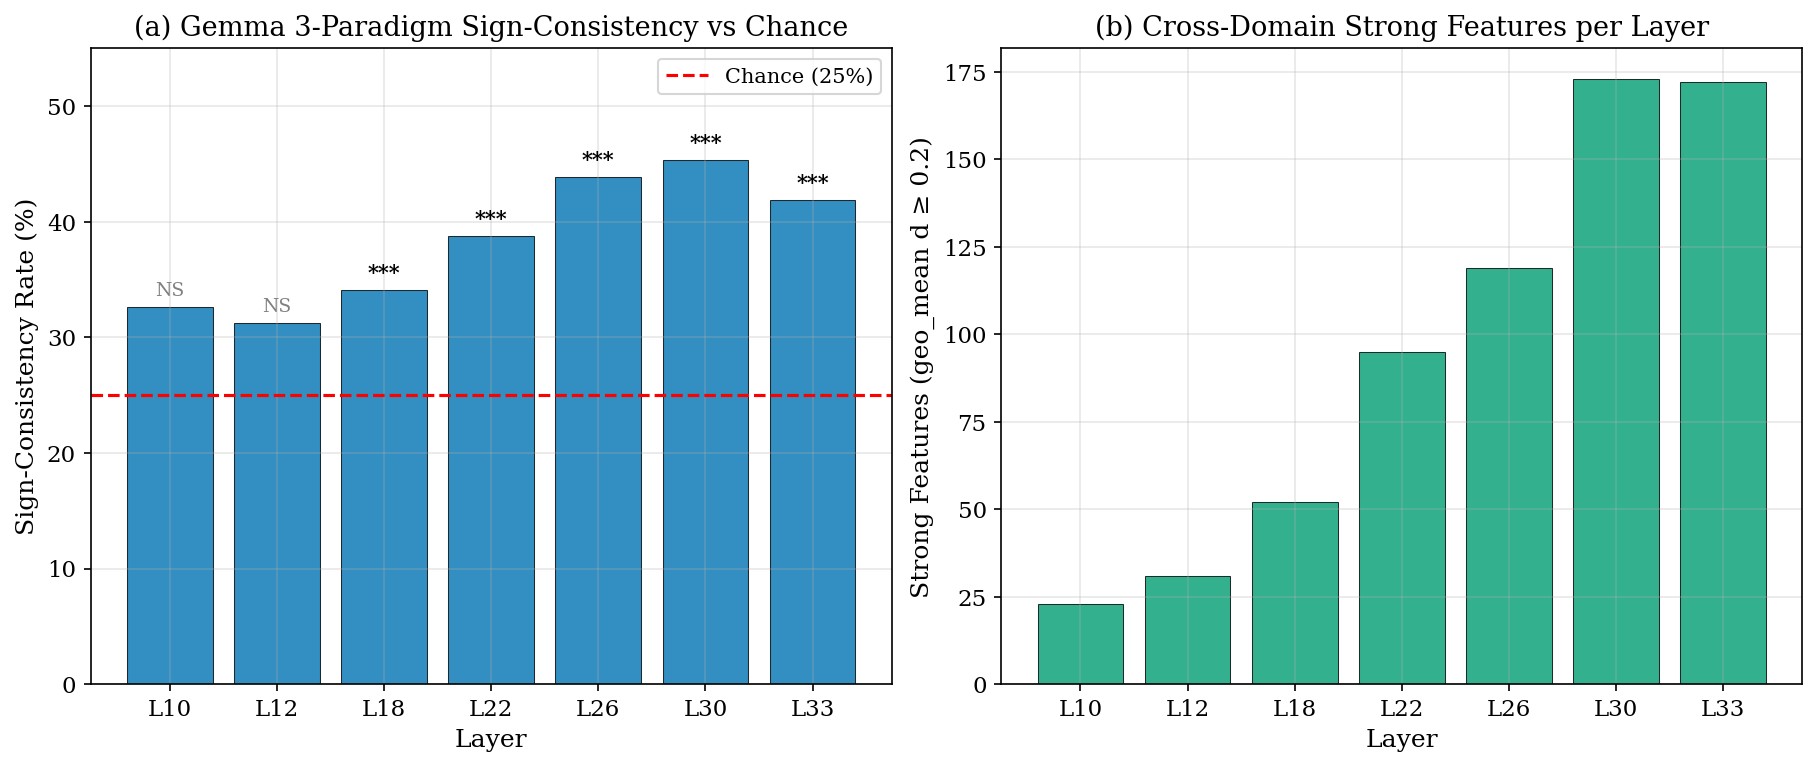
\includegraphics[width=\textwidth]{figures/fig1_crossdomain_consistency.png}
\caption{Gemma 3-paradigm sign-consistency with binomial test. L10--L12 do not exceed chance (25\%, dashed). L18+ far exceeds chance. Strong features peak at L30 (173).}
\label{fig:consistency}
\end{figure}

\subsection{Cross-Model Comparison}\label{sec:crossmodel}

\begin{table}[H]
\centering
\caption{BK Classification AUC (DP, SAE $\rightarrow$ PCA $\rightarrow$ LogReg)}\label{tab:auc}
\footnotesize
\begin{tabular}{lcc}
\toprule
Paradigm & Gemma-2-9B & LLaMA-3.1-8B \\
\midrule
SM best AUC & \textbf{0.976} (L20) & \textbf{0.974} (L8) \\
IC best AUC & \textbf{0.960} (L30) & \textbf{0.954} (L12) \\
\bottomrule
\end{tabular}
\end{table}

\begin{table}[H]
\centering
\caption{LLaMA SM AUC Across Layers}\label{tab:llama_auc}
\footnotesize
\begin{tabular}{lccc}
\toprule
Layer & AUC & n\_features & n\_BK \\
\midrule
L0  & 0.970 & 157   & 1,164 \\
L4  & 0.971 & 750   & 1,164 \\
\textbf{L8}  & \textbf{0.974} & 818   & 1,164 \\
L12 & 0.973 & 854   & 1,164 \\
L15 & 0.970 & 962   & 1,164 \\
L20 & 0.963 & 1,028 & 1,164 \\
L25 & 0.961 & 1,182 & 1,164 \\
L30 & 0.959 & 1,368 & 1,164 \\
\bottomrule
\end{tabular}
\end{table}

\begin{figure}[H]
\centering
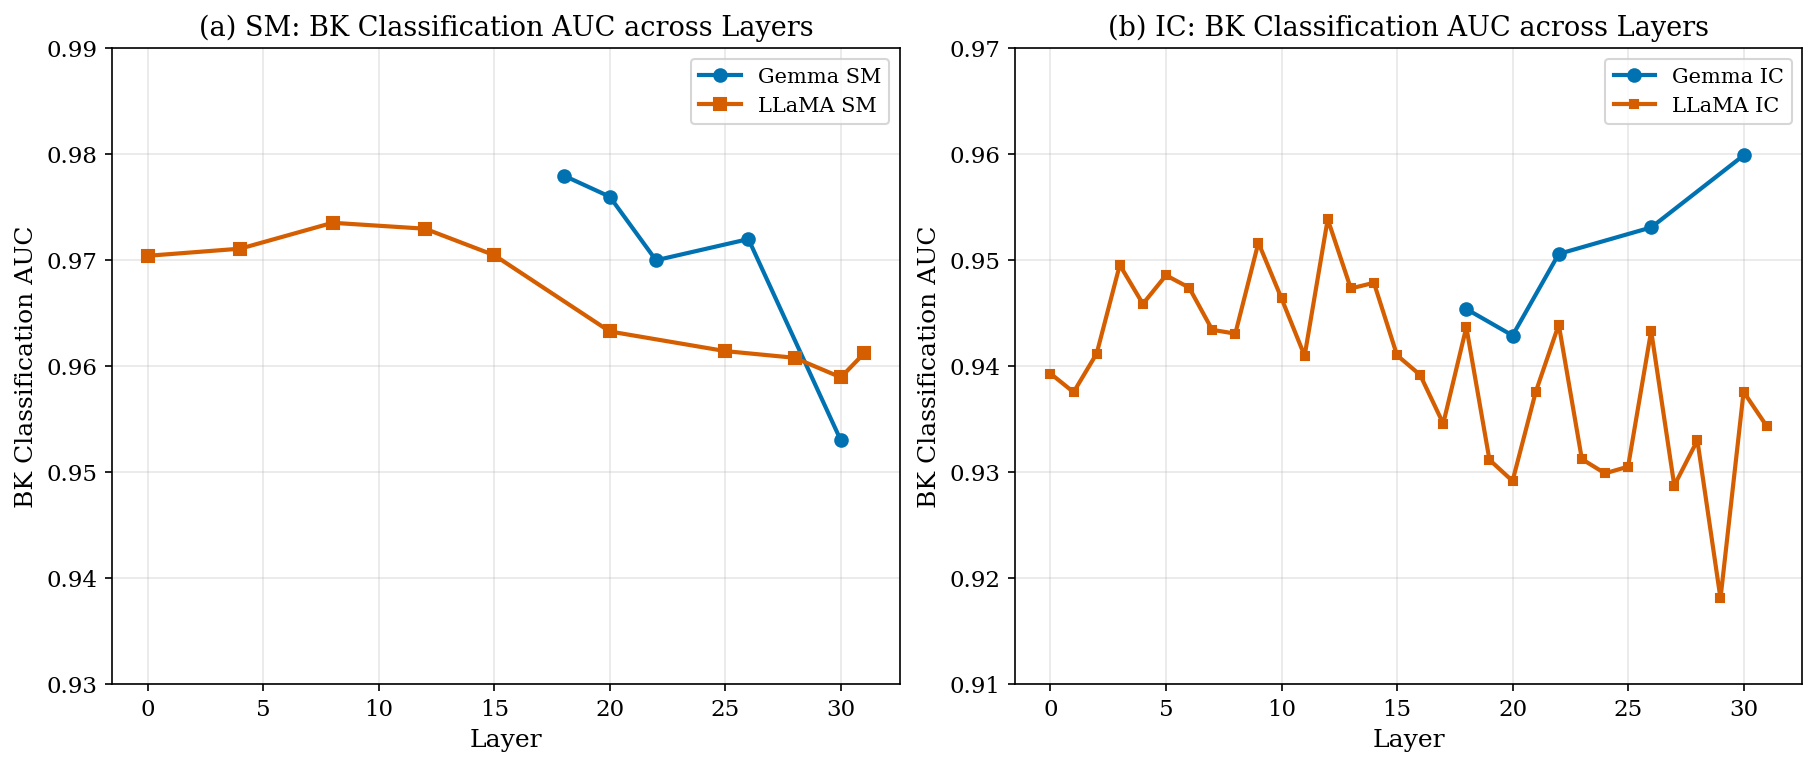
\includegraphics[width=\textwidth]{figures/fig6_classification_auc.png}
\caption{BK classification AUC across layers. (a) SM: both models AUC $> 0.95$. (b) IC: Gemma peaks L30 (0.960), LLaMA peaks L12 (0.954). Encoding depth differs but performance is near-identical.}
\label{fig:auc}
\end{figure}

\subsection{RQ1 Synthesis}

\begin{enumerate}[nosep]
    \item \textbf{Near-identical BK prediction}: 0.976 vs 0.974 (SM) --- architecture-invariant information content.
    \item \textbf{BK-inhibiting dominance at L30}: Both models (all $p < 0.001$). Not at L22 (LLaMA SM: $p=0.897$).
    \item \textbf{Encoding depth differs}: Gemma peaks mid-deep (L20), LLaMA peaks early (L8).
    \item \textbf{R1 early prediction}: AUC 0.665--0.801 from Round 1.
    \item \textbf{Factor decomposition}: 65--71\% features encode BK independently (perm $p=0.000$).
\end{enumerate}

% ============================================================
% 3. RQ2
% ============================================================
\section{RQ2: Domain Invariance}

\subsection{Hidden State Cross-Domain Transfer (Gemma L22)}

\begin{table}[H]
\centering
\caption{Hidden State vs SAE Transfer (Gemma L22)}\label{tab:hs_sae}
\footnotesize
\begin{tabular}{lcccc}
\toprule
Transfer & Hidden AUC & SAE AUC & $\Delta$ (HS$-$SAE) & HS perm\_$p$ \\
\midrule
IC $\rightarrow$ SM & \textbf{0.746} & 0.499 (NS) & +0.247 & 0.000 \\
IC $\rightarrow$ MW & \textbf{0.826} & 0.876 & $-$0.050 & 0.000 \\
SM $\rightarrow$ MW & \textbf{0.920} & 0.819 & +0.101 & 0.000 \\
\bottomrule
\end{tabular}
\end{table}

Hidden state transfer exceeds SAE in IC$\rightarrow$SM (+0.247) and SM$\rightarrow$MW (+0.101). BK signal is distributed; SAE sparsification loses coherence.

\subsection{SAE Cross-Domain Transfer (Gemma)}

\begin{table}[H]
\centering
\caption{Best SAE Transfer AUC Per Direction (Gemma)}\label{tab:sae_transfer}
\footnotesize
\begin{tabular}{lcccc}
\toprule
Transfer & Best Layer & AUC & perm\_$p$ & Null mean \\
\midrule
IC $\rightarrow$ SM & L26 & \textbf{0.913} & 0.000 & 0.498 \\
IC $\rightarrow$ MW & L18 & \textbf{0.932} & 0.000 & 0.504 \\
SM $\rightarrow$ MW & L30 & \textbf{0.867} & 0.000 & 0.504 \\
SM $\rightarrow$ IC & L30 & 0.646 & 0.000 & 0.500 \\
MW $\rightarrow$ IC & L22 & 0.853 & 0.000 & 0.500 \\
\bottomrule
\end{tabular}
\end{table}

\begin{figure}[H]
\centering
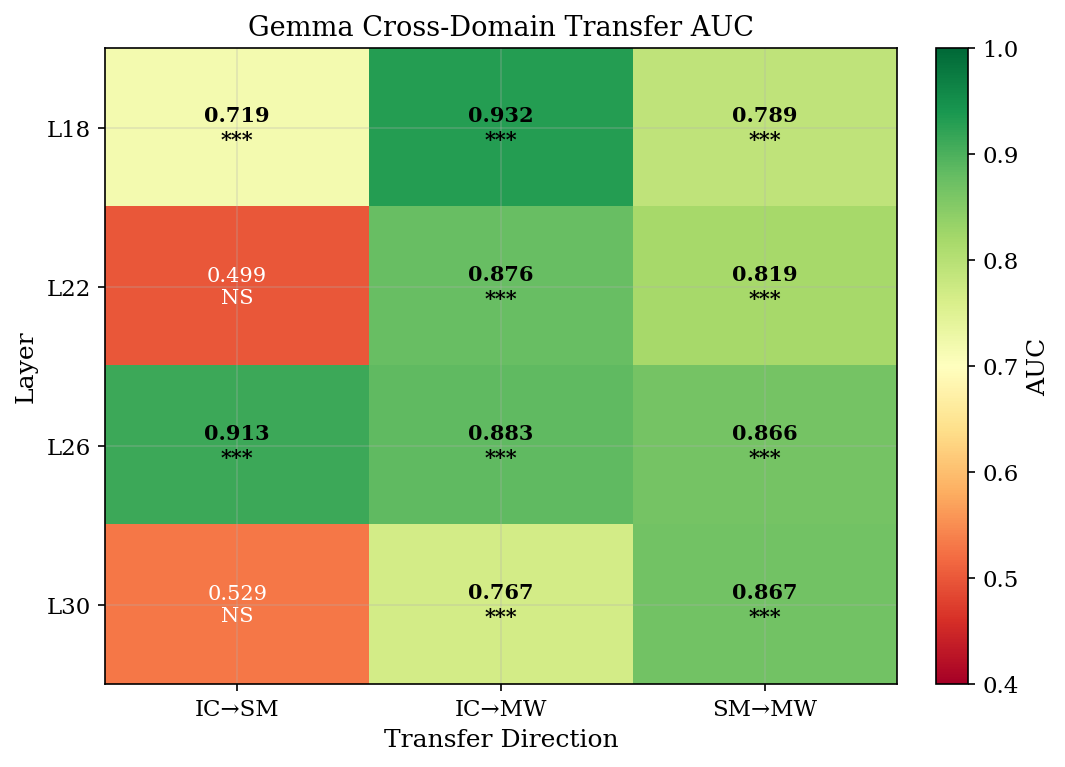
\includegraphics[width=\textwidth]{figures/fig4_transfer_heatmap.png}
\caption{Gemma cross-domain transfer heatmap. IC$\rightarrow$MW and SM$\rightarrow$MW are significant at all layers. IC$\rightarrow$SM is layer-dependent (L26: 0.913, L22: 0.499 NS).}
\label{fig:transfer}
\end{figure}

\subsection{3D Shared BK Subspace (Gemma L22)}

\begin{table}[H]
\centering
\caption{3D Shared Subspace Performance}\label{tab:3d}
\footnotesize
\begin{tabular}{lcc}
\toprule
Paradigm & 3D Subspace AUC & Full-dim AUC (50-PC) \\
\midrule
IC & 0.862 $\pm$ 0.029 & $\sim$0.95+ \\
SM & 0.899 $\pm$ 0.034 & $\sim$0.97+ \\
MW & 0.970 $\pm$ 0.016 & $\sim$0.97+ \\
\bottomrule
\end{tabular}
\end{table}

LR weight vector cosines: IC--SM=0.042, IC--MW=$-$0.026, SM--MW=$-$0.026 (near-orthogonal). Despite this, the 3D subspace achieves AUC 0.86--0.97 --- BK signal is distributed across a subspace, not a single direction.

\subsection{Factor Decomposition}

\begin{table}[H]
\centering
\caption{Factor Decomposition: Outcome-Significant Features}\label{tab:factor}
\footnotesize
\begin{tabular}{lcc}
\toprule
Factor & Gemma (581 feat., 3-par.) & LLaMA (1,418 feat., 2-par.) \\
\midrule
\textbf{Outcome} (BK) & \textbf{65.2\%} & \textbf{69.5\%} \\
Bet-type            & 92.3\% & 81.4\% \\
Paradigm            & 99.8\% & 96.2\% \\
\bottomrule
\end{tabular}
\end{table}

\begin{figure}[H]
\centering
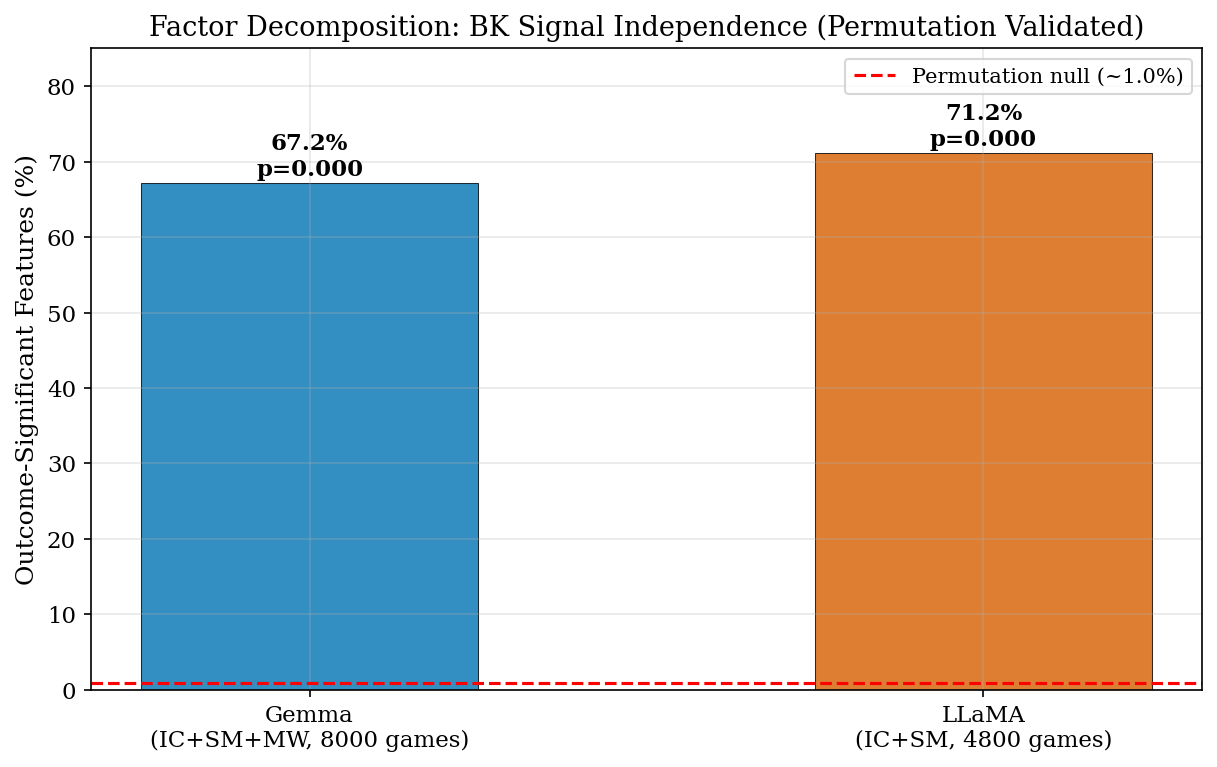
\includegraphics[width=\textwidth]{figures/fig3_factor_decomposition.png}
\caption{Factor decomposition with permutation test. Both models: 65--71\% outcome-significant (blue/orange), exceeding null ($\sim$1\%, dashed) by $60\times$+. Perm $p=0.000$.}
\label{fig:factor}
\end{figure}

\subsection{LLaMA Cross-Domain Transfer (IC $\leftrightarrow$ SM)}\label{sec:llamatransfer}

\begin{table}[H]
\centering
\caption{LLaMA IC$\leftrightarrow$SM Transfer}\label{tab:llama_transfer}
\footnotesize
\begin{tabular}{llccc}
\toprule
Transfer & Layer & AUC & perm\_$p$ & Null mean \\
\midrule
IC $\rightarrow$ SM & L25 & \textbf{0.783} & 0.000 & 0.500 \\
SM $\rightarrow$ IC & L30 & \textbf{0.685} & 0.000 & 0.498 \\
SM $\rightarrow$ IC & L12 & 0.662 & 0.000 & 0.498 \\
SM $\rightarrow$ IC & L8  & 0.624 & 0.000 & 0.499 \\
\bottomrule
\end{tabular}
\end{table}

Asymmetric: SM$\rightarrow$IC works at multiple layers; IC$\rightarrow$SM succeeds only at L25. Mirrors Gemma (IC$\rightarrow$SM layer-dependent at L26).

\subsection{LLaMA Sign-Consistency \& Within-Bet-Type}

LLaMA 2-paradigm sign-consistency: 51--57\% per layer, but chance level is 50\%. Only 3/16 layers significantly exceed chance. Raw sign-consistency is weak evidence; transfer AUC (\S\ref{sec:llamatransfer}) is more reliable.

LLaMA within-bet-type: Fixed $d$-correlation = 0.209 ($p = 1.2\times10^{-7}$) confirms Fixed cross-domain consistency. Variable $d$-correlation = $-$0.097 --- IC and SM Variable BK representations are genuinely different (bootstrap: mean=$-$0.075, 95\% CI $[-0.179, +0.032]$).

% ============================================================
% 4. RQ3
% ============================================================
\section{RQ3: Prompt Condition Effects}

\subsection{Fixed vs Variable BK Direction}\label{sec:bkdir}

\begin{table}[H]
\centering
\caption{BK Direction Cosine Similarity (Gemma IC, 3584 neurons)}\label{tab:gemma_cos}
\footnotesize
\begin{tabular}{lcccc}
\toprule
Layer & Var BK & Fix BK & $\cos(\mathrm{dir_{Var}}, \mathrm{dir_{Fix}})$ & Common neurons \\
\midrule
L10 & 14 & 158 & $-$0.195 & 178 \\
L18 & 14 & 158 & $-$0.082 & 197 \\
L22 & 14 & 158 & +0.330  & 555 \\
L26 & 14 & 158 & +0.443  & 1,053 \\
L30 & 14 & 158 & +0.401  & 1,073 \\
\bottomrule
\end{tabular}
\end{table}

\begin{table}[H]
\centering
\caption{BK Direction Cosine Similarity (LLaMA IC, 4096 neurons)}\label{tab:llama_cos}
\footnotesize
\begin{tabular}{lcc}
\toprule
Layer & $\cos(\mathrm{dir_{Var}}, \mathrm{dir_{Fix}})$ & Common neurons \\
\midrule
L8  & \textbf{0.882} & 2,513 (61.4\%) \\
L12 & \textbf{0.814} & 2,424 (59.2\%) \\
L22 & \textbf{0.835} & 2,587 (63.2\%) \\
L25 & \textbf{0.837} & 2,545 (62.1\%) \\
L30 & \textbf{0.819} & 2,488 (60.7\%) \\
\bottomrule
\end{tabular}
\end{table}

\begin{figure}[H]
\centering
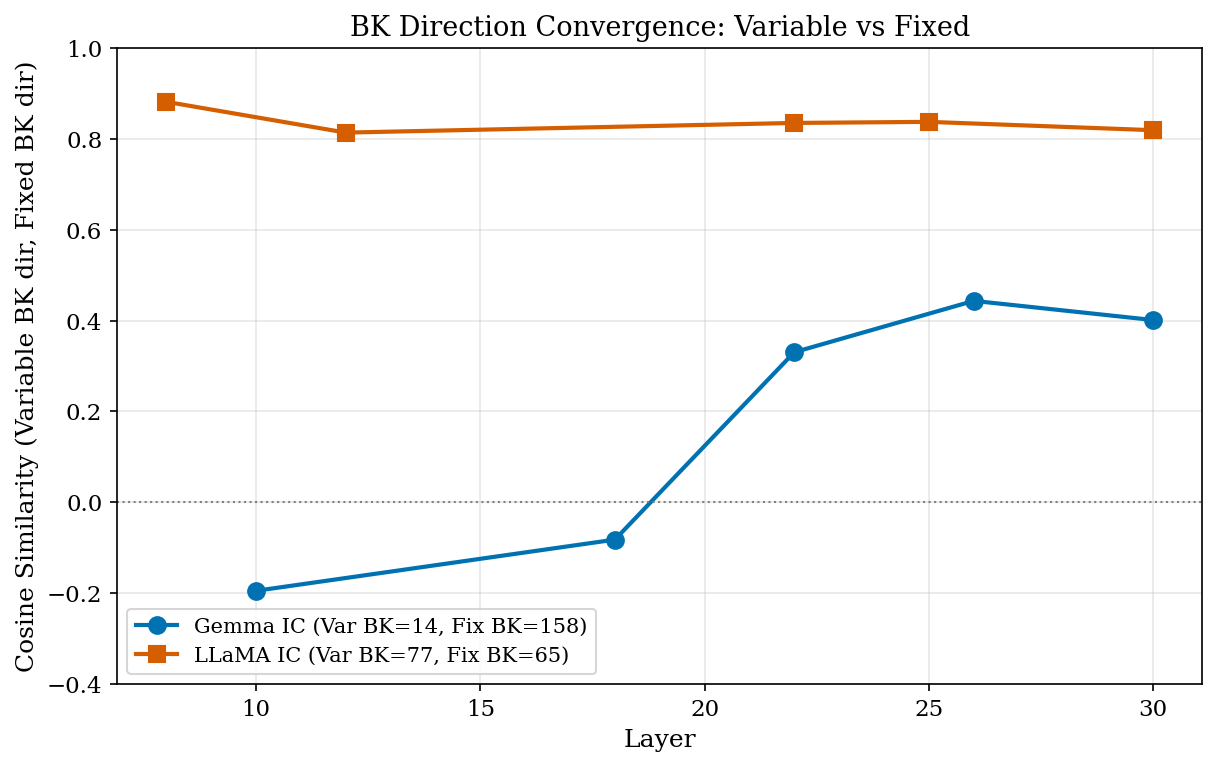
\includegraphics[width=\textwidth]{figures/fig2_bk_direction_crossmodel.png}
\caption{BK direction cosine across layers. Gemma (blue): negative at shallow, positive at deep. LLaMA (orange): $\cos > 0.81$ at all layers. Gemma's shallow negative is likely a sample-size artifact (Var BK=14).}
\label{fig:bkdir}
\end{figure}

\subsection{Shared BK Neurons (Interaction Regression)}

\begin{table}[H]
\centering
\caption{Shared BK Neurons Across Models}\label{tab:shared}
\footnotesize
\begin{tabular}{lccc}
\toprule
 & Gemma IC L22 & LLaMA IC L22 & LLaMA SM L22 \\
\midrule
$n$\_neurons      & 3,584 & 4,096 & 4,096 \\
$n$\_BK           & 172   & 142   & 1,164 \\
Outcome-sig       & 1,639 (45.7\%) & 3,150 (76.9\%) & 1,052 (25.7\%) \\
Interaction-sig   & 448 (12.5\%) & 1,605 (39.2\%) & 1,495 (36.5\%) \\
\textbf{Shared BK} & \textbf{1,182 (33.0\%)} & \textbf{1,501 (36.6\%)} & \textbf{72 (1.8\%)} \\
\bottomrule
\end{tabular}
\end{table}

\begin{figure}[H]
\centering
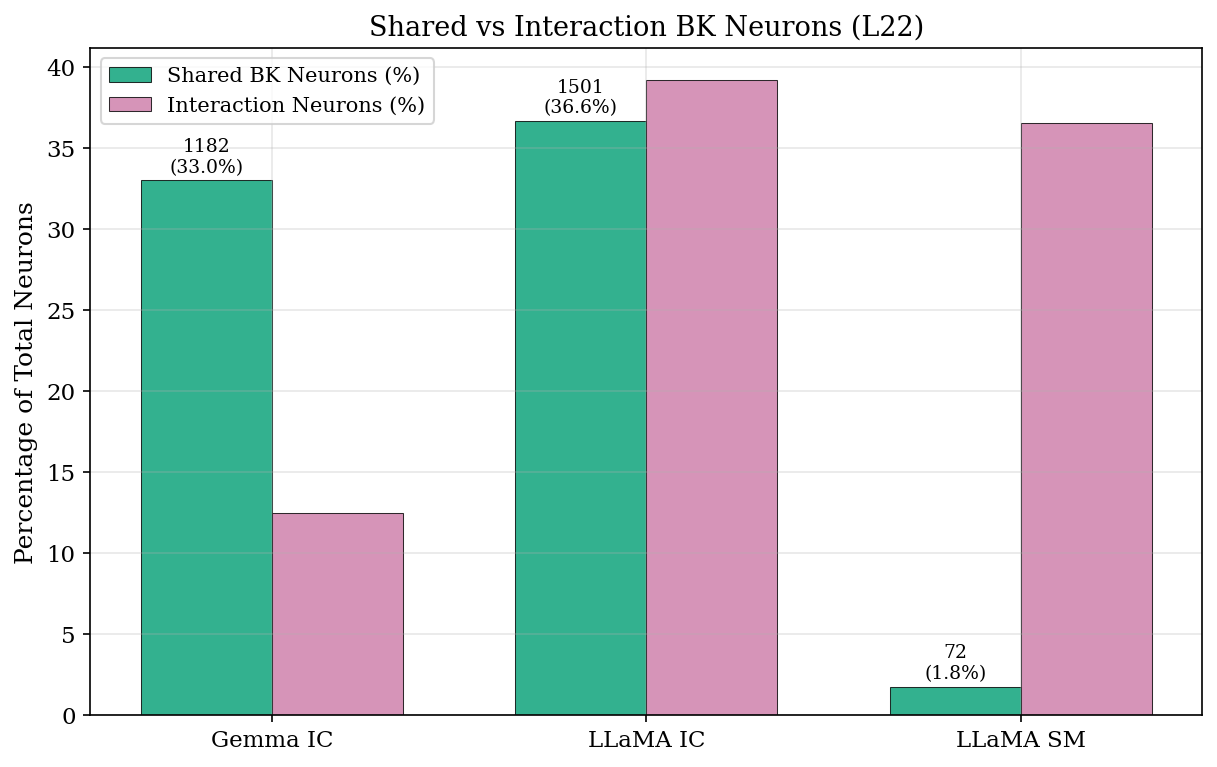
\includegraphics[width=\textwidth]{figures/fig7_shared_bk_neurons.png}
\caption{Shared vs Interaction BK neurons. Gemma IC (33.0\%) and LLaMA IC (36.6\%) show similar proportions. LLaMA SM (1.8\%) reflects Variable-dominated BK structure.}
\label{fig:shared}
\end{figure}

\subsection{Prompt Component Analysis}

\begin{table}[H]
\centering
\caption{Prompt Component BK Rate Effects (Cross-Model)}\label{tab:prompt}
\footnotesize
\begin{tabular}{lccc}
\toprule
Component & Gemma SM ratio & LLaMA SM ratio & Cross-model \\
\midrule
\textbf{G} (Goal)   & \textbf{20.75$\times$} & 1.26$\times$ & Gemma $\gg$ LLaMA \\
M (Mood/Money) & 2.35$\times$  & 1.31$\times$ & Gemma $>$ LLaMA \\
W (Warning)    & 2.35$\times$  & 1.15$\times$ & Gemma $>$ LLaMA \\
R (Reset)      & 1.72$\times$  & ---           & Gemma only \\
P (Persona)    & 1.17$\times$  & 1.06$\times$ & Both negligible \\
\bottomrule
\end{tabular}
\end{table}

\begin{figure}[H]
\centering
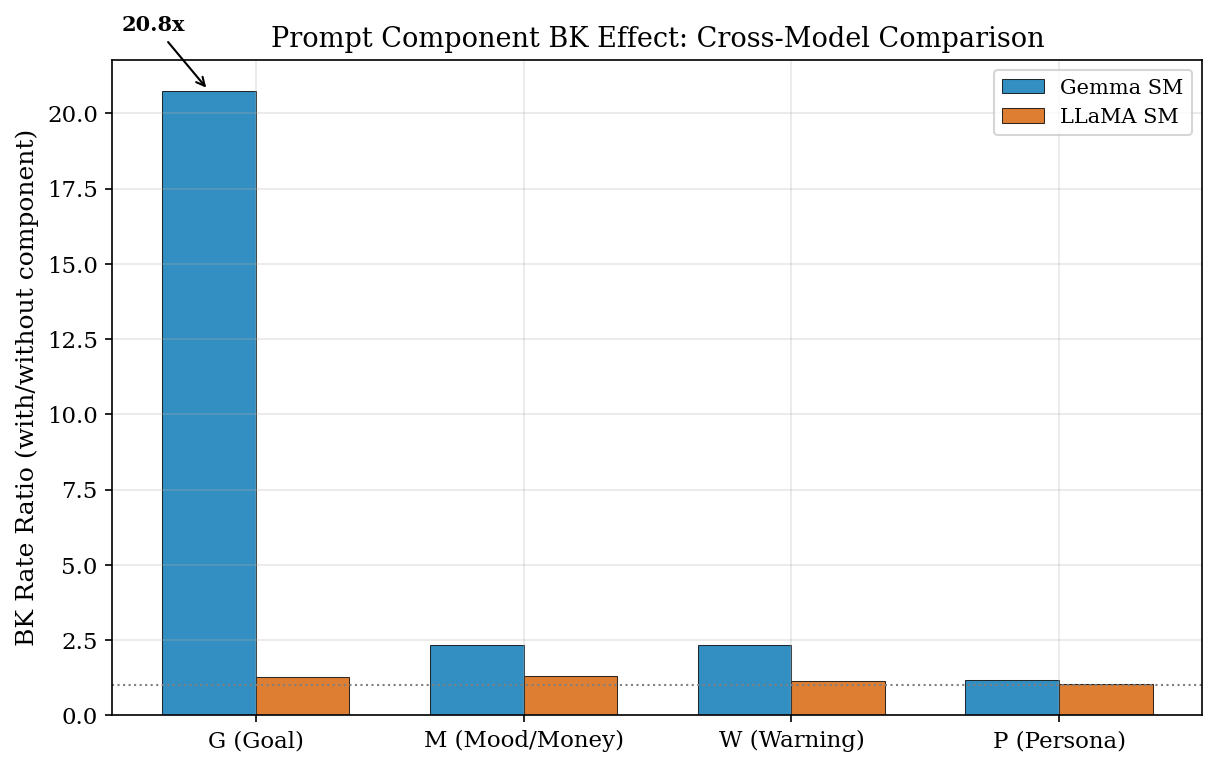
\includegraphics[width=\textwidth]{figures/fig5_prompt_components.png}
\caption{Prompt component BK effect. G(Goal) produces $20.8\times$ BK increase in Gemma (dominant) but only $1.26\times$ in LLaMA. Same prompt, $16\times$ different behavioral effect.}
\label{fig:prompt}
\end{figure}

G drives BK independently in both models (amplifies\_bk $\approx 0$ in Gemma, 8.2\% in LLaMA). Warning effects are shallow-only in both models (vanishes at deep layers). M(Money) is LLaMA's highest BK amplifier (14.5\% at L30), negligible in Gemma.

\subsection{G-Prompt Alignment \& Bet Constraint}

\textbf{G-Prompt direction alignment} (Gemma L22): SM $\cos(G, BK) = +0.850$ (strong), IC $= -0.143$, MW $= +0.367$. G pushes hidden states toward BK in SM.

\textbf{Bet constraint linear mapping} (Gemma IC L22): c10$\rightarrow$c70 maps linearly to BK-projection ($r=0.979, p=0.021$). c10: 0\% BK, c70: 21\% BK.

% ============================================================
% 5. LIMITATIONS
% ============================================================
\section{Limitations \& Critical Assessment}

\subsection{Validated vs.\ Unvalidated Claims}

\begin{table}[H]
\centering
\caption{Permutation-Validated Claims}\label{tab:validated}
\footnotesize
\begin{tabular}{lll}
\toprule
Claim & Test & Result \\
\midrule
Factor decomposition 67--71\% & 100-perm shuffle & $p=0.000$ \checkmark \\
BK-inhibiting L30 & Binomial & All $p < 0.001$ \checkmark \\
BK-inhibiting L22 & Binomial & LLaMA SM $p=0.897$ $\times$ \\
Variable cross-domain & Bootstrap & mean=$-$0.075, CI incl.\ 0 $\times$ \\
Classification AUC & 100-perm shuffle & $p=0.000$ \checkmark \\
Gemma 3-par.\ consistency & Binomial vs 25\% & L18+ $p < 5\times10^{-3}$ \checkmark \\
\bottomrule
\end{tabular}
\end{table}

\subsection{Key Limitations}

\begin{enumerate}[nosep]
    \item \textbf{LLaMA MW not extracted}: 3-paradigm cross-model comparison not possible.
    \item \textbf{Gemma IC Variable BK=14}: Very limited power for bet-type comparisons.
    \item \textbf{No causal validation}: All analyses are correlational.
    \item \textbf{Multiple comparisons}: FDR not systematically applied to all analyses.
    \item \textbf{Cross-model effect size confound}: Gemma SM $n_{BK}=87$ vs LLaMA $n_{BK}=1{,}164$ --- small-sample inflation in Gemma.
    \item \textbf{BK rate heterogeneity}: 2.7\% vs 36.4\% across models complicates comparison.
\end{enumerate}

% ============================================================
% 6. NEXT STEPS
% ============================================================
\section{Next Steps}

\begin{enumerate}[nosep]
    \item \textbf{Activation patching}: Causal validation of top cross-domain features.
    \item \textbf{LLaMA MW extraction}: Complete 3-paradigm comparison.
    \item \textbf{IC$\rightarrow$SM transfer mechanism}: Investigate layer-specific alignment.
    \item \textbf{FDR correction}: Apply to all per-feature/per-neuron tests.
    \item \textbf{G component deep dive}: Explain $20.75\times$ vs $1.26\times$ divergence.
    \item \textbf{BK rate confound control}: Balanced subsampling for IC-SM re-analysis.
\end{enumerate}

\end{document}
